\documentclass[12pt]{beamer}
\usetheme{Madrid}
\usepackage[utf8]{inputenc}
\usepackage[spanish]{babel}
\usepackage{amsmath}
\usepackage{amsfonts}
\usepackage{amssymb}
\usepackage{graphicx}
\author{Jorge Raúl Alanís Núñez \and Nohely Sarahí Fierros Méndez}
\title{"Paralelización de algoritmos de optimización para la localización espacial de plantas de producción de energía eléctrica"1}
\subtitle{{\normalsize Proyecto unidad II \\Cómputo de alto desempeño} }
\setbeamercovered{transparent} 
\setbeamertemplate{navigation symbols}{} 
%\logo{} 
\institute{Escuela Nacional de Estudios Superiores Unidad Morelia} 
%\date{} 
%\subject{} 
\begin{document}

\begin{frame}
\titlepage
\end{frame}


\begin{frame}{Antecedentes}
La herramienta de optimización PROBIOMASA sirve para la solución de problemas de localización de instalaciones, específicamente para plantas de biomasa, utilizando diversos algoritmos y heurísticas para observar la variabilidad de los resultados.\\

\begin{center}
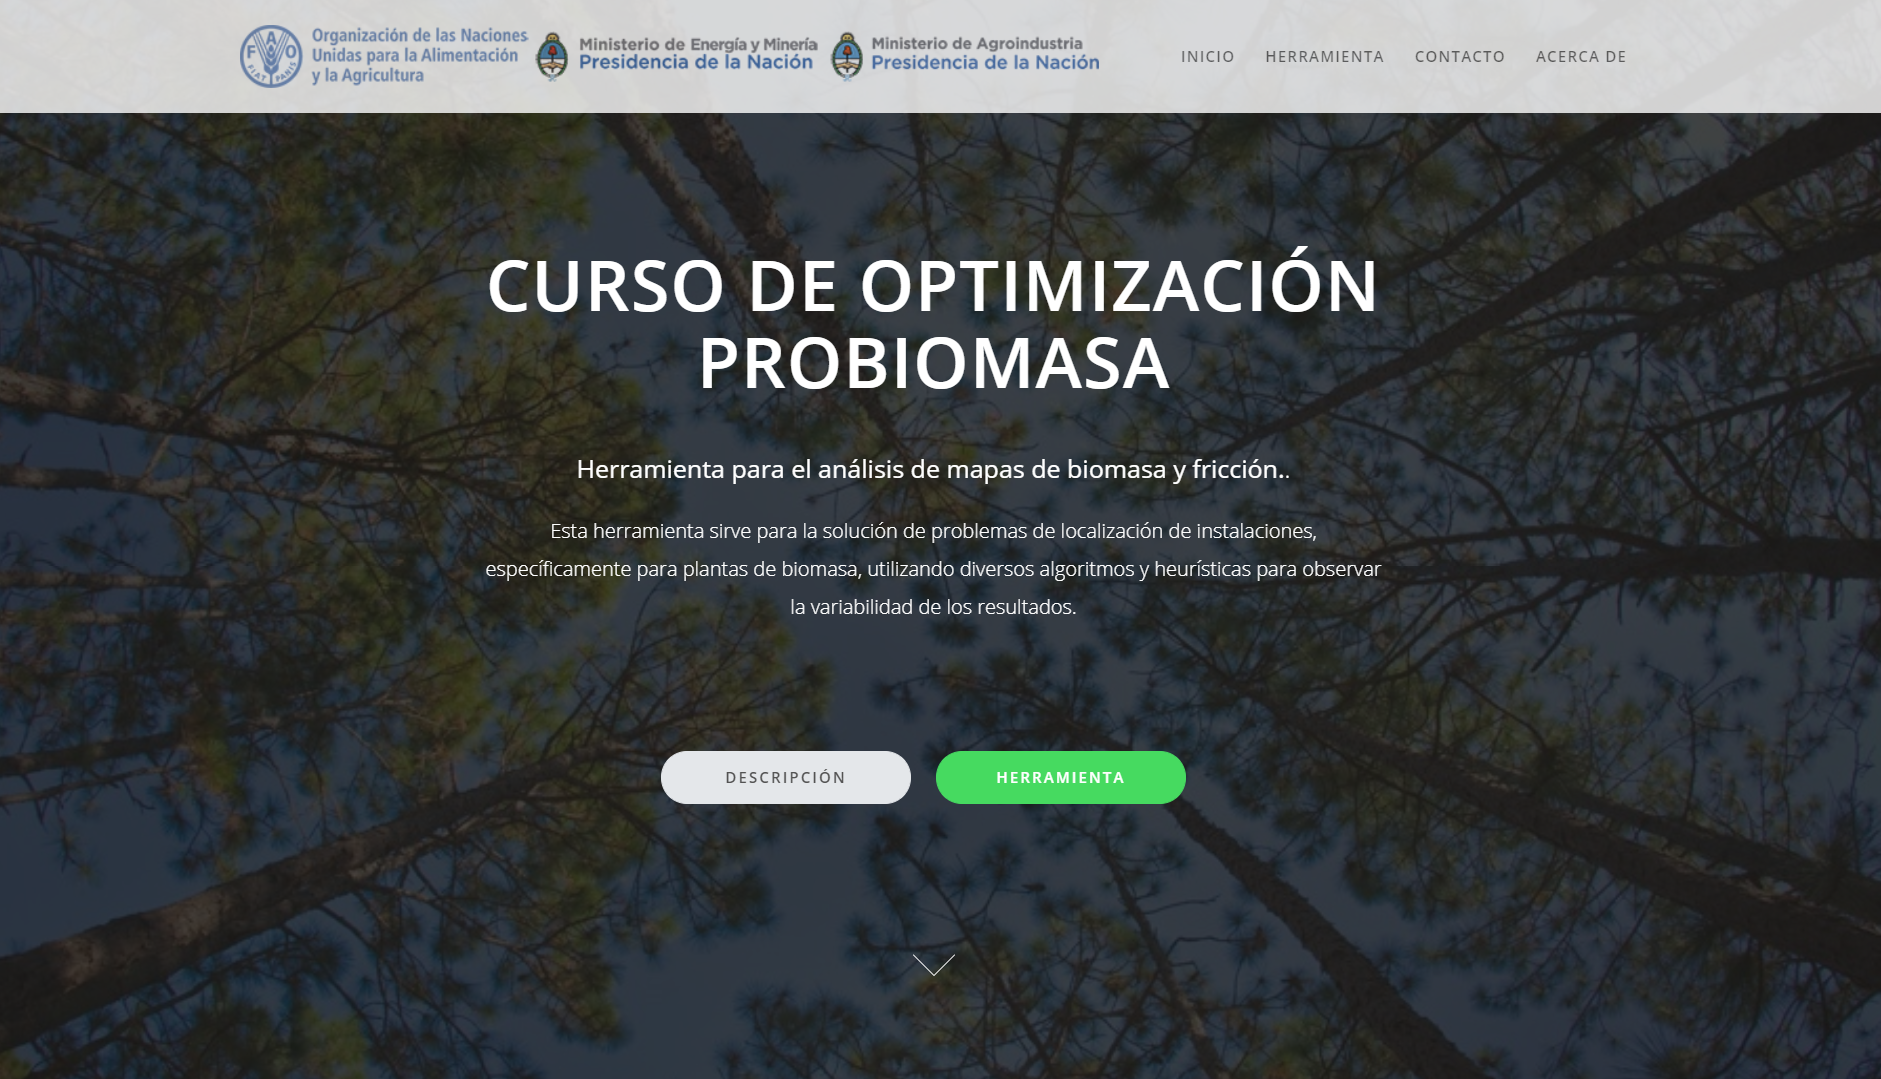
\includegraphics[width=10.0cm,height=4cm]{webpage.png}
\footnotesize\url{http://www.mofuss.unam.mx/optimization/}
\end{center}

\end{frame}

\begin{frame}{Antecedentes}
La plataforma fue desarrollada en el lenguaje de programación C++ y se utilizaron las siguientes librerías y herramientas:
\begin{itemize}
\item GDAL
\item OpenCV
\item Google Maps
\item Tclap
\item OpenMP
\end{itemize} 
\end{frame}

\begin{frame}{Función de costo distancia - movimiento nodo adyacente}
El coste de viajar de un nodo al siguiente depende de la orientación espacial de los nodos. La forma en que están conectadas las celdas también afecta el coste del viaje.\\

\begin{center}
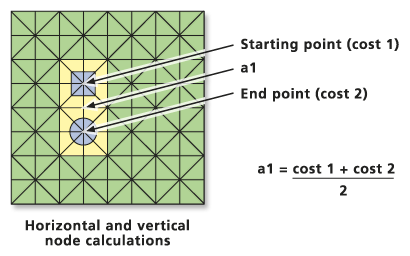
\includegraphics[scale=2]{costo1.png}
\footnotesize\url{https://desktop.arcgis.com/es/arcmap/10.3/tools/spatial-analyst-toolbox/how-the-cost-distance-tools-work.htm}
\end{center}

\end{frame}

\begin{frame}{Función de costo distancia - movimiento perpendicular acumulativo}
\begin{center}
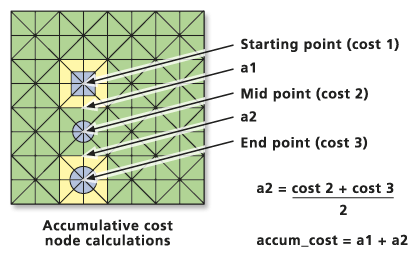
\includegraphics[scale=2]{costo2.png}
\footnotesize\url{https://desktop.arcgis.com/es/arcmap/10.3/tools/spatial-analyst-toolbox/how-the-cost-distance-tools-work.htm}
\end{center}
\end{frame}

\begin{frame}{Función de costo distancia - movimiento diagonal}
\begin{center}
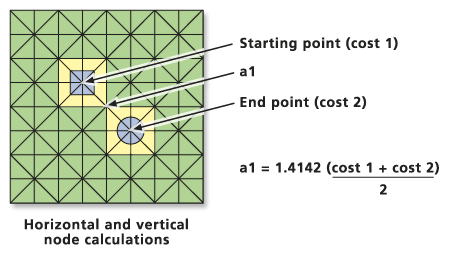
\includegraphics[scale=2]{costo3.png}
\footnotesize\url{https://desktop.arcgis.com/es/arcmap/10.3/tools/spatial-analyst-toolbox/how-the-cost-distance-tools-work.htm}
\end{center}
\end{frame}

\begin{frame}{Función de costo distancia - iteración del raster de coste aumulativo}
\begin{center}
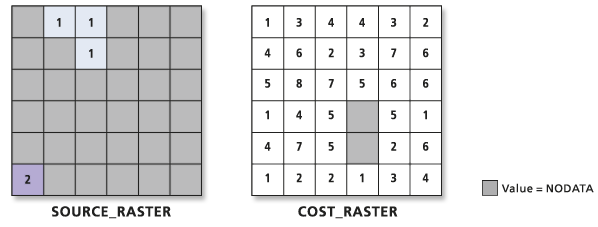
\includegraphics[scale=2]{costo4.png}
\footnotesize\url{https://desktop.arcgis.com/es/arcmap/10.3/tools/spatial-analyst-toolbox/how-the-cost-distance-tools-work.htm}
\end{center}
\end{frame}

\begin{frame}{Función de costo distancia - iteración del raster de coste aumulativo}
\begin{center}
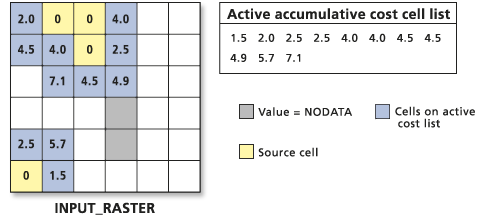
\includegraphics[scale=2]{costo5.png}
\footnotesize\url{https://desktop.arcgis.com/es/arcmap/10.3/tools/spatial-analyst-toolbox/how-the-cost-distance-tools-work.htm}
\end{center}
\end{frame}

\begin{frame}{Función de costo distancia - iteración del raster de coste aumulativo}
\begin{center}
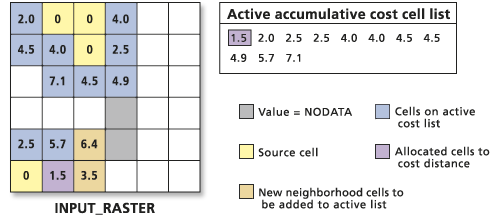
\includegraphics[scale=2]{costo6.png}
\footnotesize\url{https://desktop.arcgis.com/es/arcmap/10.3/tools/spatial-analyst-toolbox/how-the-cost-distance-tools-work.htm}
\end{center}
\end{frame}

\begin{frame}{Función de costo distancia - raster final}
\begin{center}
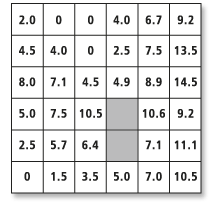
\includegraphics[scale=3]{costo7.png}
\footnotesize\url{https://desktop.arcgis.com/es/arcmap/10.3/tools/spatial-analyst-toolbox/how-the-cost-distance-tools-work.htm}
\end{center}
\end{frame}

\begin{frame}{Objetivos}
\begin{itemize}
\item Paralelizar la función de costo distancia.
\item Paralelizar la exploración del algoritmo de optimización.\\

\includegraphics[scale=.1]{openmp.png} 
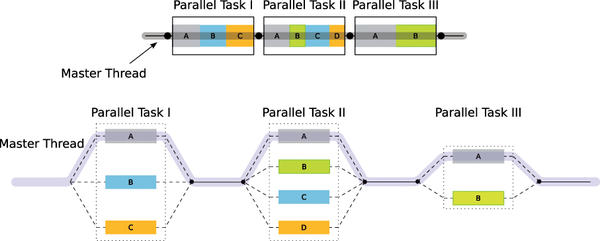
\includegraphics[scale=.3]{openmp2.jpg}
\end{itemize}

\end{frame}



\end{document}